%==========================================================================

\begin{frame}[fragile]

  {\Huge Views}

  \vspace{20pt}

  \textbf{Learning objectives:}
  \begin{itemize}
    \item{Motivation behind the \texttt{View} abstraction.}
    \item{Key \texttt{View} concepts and template parameters.}
    \item{The \texttt{View} life cycle.}
  \end{itemize}

  \vspace{-20pt}

\end{frame}

%==========================================================================

\begin{frame}[fragile]{View motivation}

  \textbf{\ul{Example: running vector addition on the GPU:}}

  \vspace{5pt}

  \begin{code}[linebackgroundcolor={
        \btLstHL<2->{3}{red!30}
      },
      frame=single
    ]
double * x = new double[N]; // also y
parallel_for("Vector-Add",N, [=] (const int64_t i) {
    y[i] += x[i];
  });
  \end{code}

  \begin{code}[linebackgroundcolor={
        \btLstHL<2->{2,4}{red!30}
      },
      frame=single
    ]
struct Functor {
  double *x_, *y_, a;
  void operator()(const int64_t i) const {
    y_[i] += x_[i];
  }
};
  \end{code}

  \begin{textblock*}{0.5\textwidth}(0.05\textwidth,0.225\textheight)
    \rotatebox{90}{\textbf{Lambda}}
  \end{textblock*}

  \begin{textblock*}{0.5\textwidth}(0.05\textwidth,0.470\textheight)
    \rotatebox{90}{\textbf{Functor}}
  \end{textblock*}

  \vspace{5pt}
  \pause

  \textbf{{\color{red}Problem}}: \texttt{x} and \texttt{y} reside in CPU memory.

  \vspace{5pt}

  Possibly accessible on an accelerator (GPU) via Heterogenous Memory Management (HMM) but it will be inefficient.

  \vspace{10pt}

\end{frame}

%==========================================================================

\begin{frame}[fragile]{Views (0)}

  {\Large \textbf{What do we need?}}

  \vspace{10pt}

  A way to manage data (multidimensional arrays) in a heterogeneous computing system.

  \vspace{10pt}

  {\Large $\Rightarrow$ \textbf{Views}}

\end{frame}

%==========================================================================

\begin{frame}[fragile]{Views (1)}

  \ul{\textbf{View} abstraction}
  \begin{itemize}
  \item {A \textit{lightweight} C\texttt{++} class with a pointer to array data and a little meta-data,}
  \item {that is \textit{templated} on the data type (and other things).}
  \end{itemize}

  \vspace{5pt}

  \ul{\textbf{High-level example} of Views for vector addition using lambda}:

  \begin{code}[frame=single, keywords={}]
@blueView<double*, ...>@blue x(...), y(...);
@gray...populate x, y... @gray

parallel_for("Vector-Add",N, [=] (const int64_t i) {
    // Views x and y captured by value; data not copied
    y(i) += x(i);
  });
  \end{code}

  \pause
  \vspace{0pt}

  \begin{block}{Important point}
    Views are \textbf{like shared pointers}, so copy them in your functors.
  \end{block}

  \vspace{5pt}

\end{frame}

%==========================================================================

\begin{frame}[fragile]{Views (2)}

  \ul{\textbf{View} overview:}

  \begin{itemize}
    \item{\textbf{Multi-dimensional array} of 0 or more dimensions \\
          \hspace{20pt}scalar (0), vector (1), matrix (2), etc.}
    \item{\textbf{Number of dimensions (rank)} is fixed at compile-time.}
    \item{Arrays are \textbf{rectangular}, not ragged.}
    \item{\textbf{Sizes of dimensions} set at compile-time or runtime. \\
          \hspace{20pt}e.g., 2x20, 50x50, etc.}
    \item{Access elements via "(...)" operator.}
  \end{itemize}

  \pause
  \vspace{-3pt}

  \textbf{Example}:
  \vspace{-3pt}
  \begin{code}[keywords={double,View}]
View<double***> data("label", N0, N1, N2); //<@3 run, 0 compile@>
View<double**[N2]> data("label", N0, N1);  //<@2 run, 1 compile@>
View<double*[N1][N2]> data("label", N0);   //<@1 run, 2 compile@>
View<double[N0][N1][N2]> data("label");    //<@0 run, 3 compile@>
//Access
data(i,j,k) = 5.3;
  \end{code}

  \vspace{-1pt}
  Note: runtime-sized dimensions must come first.

\end{frame}

%==========================================================================

\begin{frame}[fragile]{Views (3)}

  \ul{\textbf{View} life cycle:}

  \begin{itemize}
    \item{Allocations only happen when \emph{explicitly} specified. \\
          \hspace{20pt}i.e., there are \textbf{no hidden allocations}.}
    \item{Behaviour is like \texttt{std::shared\_ptr}. \\
          \hspace{20pt}i.e., shared ownership semantics.}
    \item{Reference counting is used for \textbf{automatic deallocation.}}
    \item{Copy construction and assignment are \textbf{shallow}. \\
          \hspace{20pt}i.e., the data pointed to is not copied.}
    \item{For clear semantics: pass \texttt{Views} by value, \emph{not} by reference}.
  \end{itemize}

\end{frame}

%==========================================================================

\begin{frame}[fragile,t]{Views (4)}

  \textbf{Example}:

  % ---------- Top half: images ----------
  \begin{textblock*}{0.9\textwidth}(0.05\textwidth,0.20\textheight)
    \centering
    \only<1>{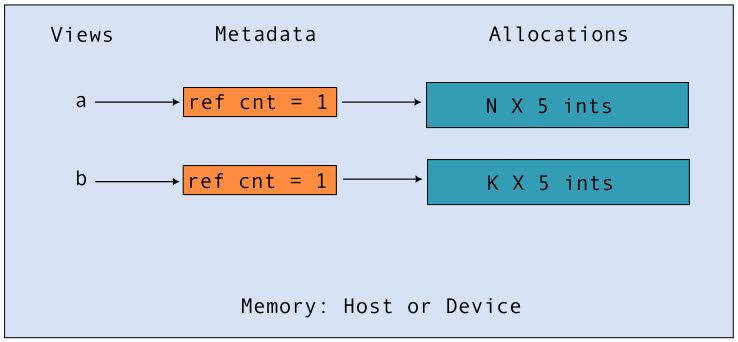
\includegraphics[height=0.32\textheight]{figures/view-copy-a-b-diff.png}}
    \only<2>{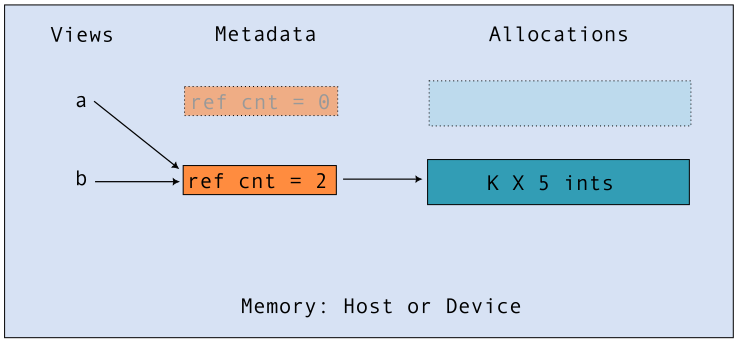
\includegraphics[height=0.32\textheight]{figures/view-copy-a-b-same.png}}
    \only<3->{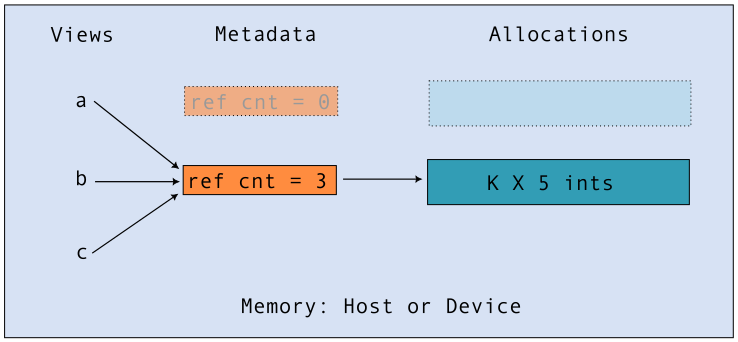
\includegraphics[height=0.32\textheight]{figures/view-copy-a-b-c.png}}
  \end{textblock*}

  % ---------- Bottom half: code ----------
  \begin{textblock*}{0.95\textwidth}(0.05\textwidth,0.56\textheight)
    \begin{onlyenv}<1>
      \begin{code}[keywords={}]
View<double*[5]> @bluea@blue("a", N), @darkgreenb@darkgreen("b", K);
      \end{code}
    \end{onlyenv}
    \begin{onlyenv}<2>
      \begin{code}[keywords={}]
View<double*[5]> @bluea@blue("a", N), @darkgreenb@darkgreen("b", K);
@bluea@blue = @darkgreenb@darkgreen;
      \end{code}
    \end{onlyenv}
    \begin{onlyenv}<3>
      \begin{code}[keywords={}]
View<double*[5]> @bluea@blue("a", N), @darkgreenb@darkgreen("b", K);
@bluea@blue = @darkgreenb@darkgreen;
View<double**> @darkredc@darkred(@darkgreenb@darkgreen);
      \end{code}
    \end{onlyenv}
    \begin{onlyenv}<4->
      \begin{code}[keywords={}]
View<double*[5]> @bluea@blue("a", N), @darkgreenb@darkgreen("b", K);
@bluea@blue = @darkgreenb@darkgreen;
View<double**> @darkredc@darkred(@darkgreenb@darkgreen);
@bluea@blue(0,2) = 1;
@darkgreenb@darkgreen(0,2) = 2;
@darkredc@darkred(0,2) = 3;
print_value( @bluea@blue(0,2) );
      \end{code}
    \end{onlyenv}
  \end{textblock*}

  % ---------- Question (step 4) ----------
  \begin{textblock*}{0.5\textwidth}(0.6\textwidth,0.78\textheight)
    \onslide<4->{What gets printed?}
  \end{textblock*}

  % ---------- Answer (step 5) ----------
  \begin{textblock*}{0.5\textwidth}(0.65\textwidth,0.83\textheight)
    \onslide<5->{\texttt{3.0}}
  \end{textblock*}

\end{frame}

%==========================================================================

\begin{frame}[fragile]{Views (5)}

  \ul{\textbf{View} Properties:}

  \begin{itemize}
    \item Accessing a \texttt{View}'s sizes is done via its \texttt{extent(dim)} function.
         \begin{itemize}
		 \item Static extents can \emph{additionally} be accessed via \texttt{static\_extent(dim)}.
	 \end{itemize}
    \item You can retrieve a raw pointer via its \texttt{data()} function.
    \item The label can be accessed via \texttt{label()}.
  \end{itemize}

  \textbf{Example}:

  \begin{code}[keywords={View,extent,static_extent,data,label,rank,is_allocated}]
	  View<double*[5]> a("A",N0);
	  static_assert(a.rank() == 2);
	  static_assert(a.is_allocated());
	  assert(a.extent(0) == N0);
	  assert(a.extent(1) == 5);
	  static_assert(a.static_extent(1) == 5);
	  assert(a.label() == "A");
  \end{code}

  {\small Refer: \href{https://kokkos.org/kokkos-core-wiki/API/core/view/view.html}{https://kokkos.org/kokkos-core-wiki/API/core/view/view.html}}

\end{frame}
%==========================================================================

\begin{frame}[fragile]{Exercise \#2: Inner Product, Flat Parallelism on the CPU, with Views}

  \begin{small}
  \begin{itemize}
  \item Location: \ExerciseDirectory{02/Begin}
  \item Assignment: Change data storage from arrays to Views.
  \end{itemize}
  \end{small}

\begin{code}
# CPU-only using OpenMP
cmake -B build_openmp -DKokkos_ENABLE_OPENMP=ON
cmake --build build_openmp
# Run exercise
./build_openmp/02_Exercise -S 26
# Note the warnings, set appropriate environment variables
\end{code}

  \begin{scriptsize}
  \begin{itemize}
  \item Vary problem size: \textbf{-S \#}
  \item Vary number of rows: \textbf{-M \#}
  \item Vary repeats: \textbf{-nrepeat \#}
  \item Advanced: add `Kokkos::SharedSpace` template parameter to View's and compile for GPUs
  \end{itemize}
  \end{scriptsize}

\end{frame}

%==========================================================================

\iffull
\begin{frame}[fragile]{Advanced features covered later}

  \begin{itemize}

  \item {\textbf{Memory space} in which view's data resides}

  \item {\textbf{deep\_copy} view's data; \\
        Note: Kokkos \textit{never} hides a deep\_copy of data.}

  \item {\textbf{Layout} of multidimensional arrays.}

  \item {\textbf{Memory traits} to control access modalities.}

  \item {\textbf{Subview}: Generating a view that is a ``slice'' of another multidimensional view.}

  \end{itemize}

\end{frame}
\fi

